% -*- coding: utf-8 -*-
%-------------------------designed by zcf--------------
\documentclass[UTF8,a4paper,10pt]{ctexart}
\usepackage[left=3.17cm, right=3.17cm, top=2.74cm, bottom=2.74cm]{geometry}
\usepackage{amsmath}
\usepackage{graphicx,subfig}
\usepackage{float}
\usepackage{cite}
\usepackage{caption}
\usepackage{enumerate}
\usepackage{booktabs} %表格
\usepackage{multirow}
\usepackage{pythonhighlight}
\newcommand{\tabincell}[2]{\begin{tabular}{@{}#1@{}}#2\end{tabular}}  %表格强制换行
%-------------------------字体设置--------------
\usepackage{times} 
\newcommand{\yihao}{\fontsize{26pt}{36pt}\selectfont}           % 一号, 1.4 倍行距
\newcommand{\erhao}{\fontsize{22pt}{28pt}\selectfont}          % 二号, 1.25倍行距
\newcommand{\xiaoer}{\fontsize{18pt}{18pt}\selectfont}          % 小二, 单倍行距
\newcommand{\sanhao}{\fontsize{16pt}{24pt}\selectfont}  %三号字
\newcommand{\xiaosan}{\fontsize{15pt}{22pt}\selectfont}        % 小三, 1.5倍行距
\newcommand{\sihao}{\fontsize{14pt}{21pt}\selectfont}            % 四号, 1.5 倍行距
\newcommand{\banxiaosi}{\fontsize{13pt}{19.5pt}\selectfont}    % 半小四, 1.5倍行距
\newcommand{\xiaosi}{\fontsize{12pt}{18pt}\selectfont}            % 小四, 1.5倍行距
\newcommand{\dawuhao}{\fontsize{11pt}{11pt}\selectfont}       % 大五号, 单倍行距
\newcommand{\wuhao}{\fontsize{10.5pt}{15.75pt}\selectfont}    % 五号, 单倍行距
%-------------------------章节名----------------
\usepackage{ctexcap} 
\CTEXsetup[name={,、},number={ \chinese{section}}]{section}
\CTEXsetup[name={(,)},number={\chinese{subsection}}]{subsection}
\CTEXsetup[name={,.},number={\arabic{subsubsection}}]{subsubsection}
%-------------------------页眉页脚--------------
\usepackage{fancyhdr}
\pagestyle{fancy}
\lhead{\kaishu \leftmark}
% \chead{}
\rhead{\kaishu 深度学习及应用作业}%加粗\bfseries 
\lfoot{}
\cfoot{\thepage}
\rfoot{}
\renewcommand{\headrulewidth}{0.1pt}  
\renewcommand{\footrulewidth}{0pt}%去掉横线
\newcommand{\HRule}{\rule{\linewidth}{0.5mm}}%标题横线
\newcommand{\HRulegrossa}{\rule{\linewidth}{1.2mm}}
%-----------------------伪代码------------------
\usepackage{algorithm}  
\usepackage{algorithmicx}  
\usepackage{algpseudocode}  
\floatname{algorithm}{Algorithm}  
\renewcommand{\algorithmicrequire}{\textbf{Input:}}  
\renewcommand{\algorithmicensure}{\textbf{Output:}} 
\usepackage{lipsum}  
\makeatletter
\newenvironment{breakablealgorithm}
  {% \begin{breakablealgorithm}
  \begin{center}
     \refstepcounter{algorithm}% New algorithm
     \hrule height.8pt depth0pt \kern2pt% \@fs@pre for \@fs@ruled
     \renewcommand{\caption}[2][\relax]{% Make a new \caption
      {\raggedright\textbf{\ALG@name~\thealgorithm} ##2\par}%
      \ifx\relax##1\relax % #1 is \relax
         \addcontentsline{loa}{algorithm}{\protect\numberline{\thealgorithm}##2}%
      \else % #1 is not \relax
         \addcontentsline{loa}{algorithm}{\protect\numberline{\thealgorithm}##1}%
      \fi
      \kern2pt\hrule\kern2pt
     }
  }{% \end{breakablealgorithm}
     \kern2pt\hrule\relax% \@fs@post for \@fs@ruled
  \end{center}
  }
\makeatother
%------------------------代码-------------------
\usepackage{xcolor} 
\usepackage{listings} 
\lstset{ 
breaklines,%自动换行
basicstyle=\small,
escapeinside=``,
keywordstyle=\color{ blue!70} \bfseries,
commentstyle=\color{red!50!green!50!blue!50},% 
stringstyle=\ttfamily,% 
extendedchars=false,% 
linewidth=\textwidth,% 
numbers=left,% 
numberstyle=\tiny \color{blue!50},% 
frame=trbl% 
rulesepcolor= \color{ red!20!green!20!blue!20} 
}
%------------超链接----------
\usepackage[colorlinks,linkcolor=black,anchorcolor=blue]{hyperref}
%------------------------TODO-------------------
\usepackage{enumitem,amssymb}
\newlist{todolist}{itemize}{2}
\setlist[todolist]{label=$\square$}
% for check symbol 
\usepackage{pifont}
\newcommand{\cmark}{\ding{51}}%
\newcommand{\xmark}{\ding{55}}%
\newcommand{\done}{\rlap{$\square$}{\raisebox{2pt}{\large\hspace{1pt}\cmark}}\hspace{-2.5pt}}
\newcommand{\wontfix}{\rlap{$\square$}{\large\hspace{1pt}\xmark}}
%------------------------水印-------------------
\usepackage{tikz}
\usepackage{xcolor}
\usepackage{eso-pic}

\newcommand{\watermark}[3]{\AddToShipoutPictureBG{
\parbox[b][\paperheight]{\paperwidth}{
\vfill%
\centering%
\tikz[remember picture, overlay]%
  \node [rotate = #1, scale = #2] at (current page.center)%
    {\textcolor{gray!80!cyan!30!magenta!30}{#3}};
\vfill}}}



%———————————————————————————————————————————正文———————————————————————————————————————————————
%----------------------------------------------
\begin{document}
\begin{titlepage}
    \begin{center}
    
\includegraphics[width=0.8\textwidth]{NKU.png}\\[1cm]    
    \textsc{\Huge \kaishu{\textbf{南\ \ \ \ \ \ 开\ \ \ \ \ \ 大\ \ \ \ \ \ 学}} }\\[0.9cm]
    \textsc{\huge \kaishu{\textbf{计\ \ 算\ \ 机\ \ 学\ \ 院}}}\\[0.5cm]
    \textsc{\Large \textbf{深度学习及应用实验作业}}\\[0.8cm]
    \HRule \\[0.9cm]
    { \LARGE \bfseries 作业一 \  前馈神经网络实践}\\[0.4cm]
    \HRule \\[2.0cm]
    \centering
    \textsc{\LARGE \kaishu{姓名\ :\ 王泳鑫}}\\[0.5cm]
    \textsc{\LARGE \kaishu{学号\ :\ 1911479}}\\[0.5cm]
    \textsc{\LARGE \kaishu{年级\ :\ 2019级}}\\[0.5cm]
    \textsc{\LARGE \kaishu{专业\ :\ 计算机科学与技术}}\\[0.5cm]
    \textsc{\LARGE \kaishu{指导教师\ :\ 侯淇彬}}\\[0.5cm]
    \vfill
    {\Large \today}
    \end{center}
\end{titlepage}
%-------------摘------要--------------
\newpage
\thispagestyle{empty}
\renewcommand{\abstractname}{\kaishu \sihao \textbf{摘要}}
    \begin{abstract}
        本次实验基于pyotch1.9,采用前馈神经网络完成手写数字识别实验并进行调参优化。
        \noindent  %顶格
        \textbf{\\\ 关键字:前馈神经网络,pytorch,FNN}\textbf{} \\\ \\\
    \end{abstract}
%----------------------------------------------------------------
\tableofcontents
%----------------------------------------------------------------
\newpage
\watermark{60}{10}{NKU}
\setcounter{page}{1}
%——————————————————————————————————————


\section{实验要求}

\begin{itemize}
    \item 掌握PyTorch框架基础算子操作
    \item 学会使用PyTorch搭建简单的前馈神经网络来训练MNIST数据集
    \item 了解如何改进网络结构、调试参数以提升网络识别性能
\end{itemize}

\section{MLP修改过程}


\subsection{加一层中间层}
在老师给出的KNN实验指导中里面只有一个中间层,在这里我又加入一个dropout为0.2的中间层,网络结果如下:


\begin{python}
class Net(nn.Module):
    def __init__(self):
        super(Net, self).__init__()
        self.fc1 = nn.Linear(28*28, 100)
        self.fc1_drop = nn.Dropout(0.2)
        self.fc2 = nn.Linear(100, 50)
        self.fc2_drop = nn.Dropout(0.2)
        self.fc3 = nn.Linear(50, 50)
        self.fc3_drop = nn.Dropout(0.2)
        self.fc4 = nn.Linear(50, 10)

    def forward(self, x):
        x = x.view(-1, 28*28)
        x = F.relu(self.fc1(x))
        x = self.fc1_drop(x)
        x = F.relu(self.fc2(x))
        x = self.fc2_drop(x)
        x = F.relu(self.fc3(x))
        x = self.fc3_drop(x)
        return F.log_softmax(self.fc4(x), dim=1)
\end{python}

\subsection{实验结果}

如图\ref{fig:1}所示
\begin{figure}[H]
    \centering
    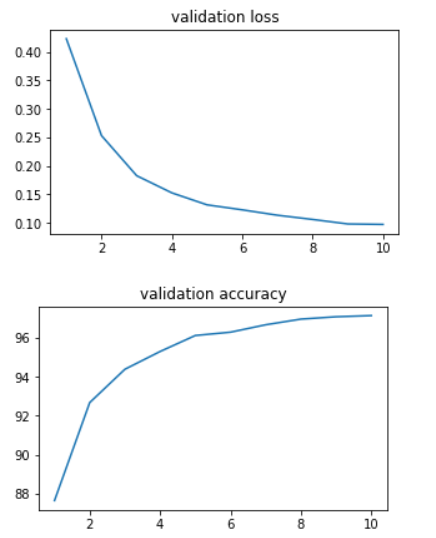
\includegraphics[scale=0.3]{2.png}
    \caption{Caption}
    \label{fig:1}
\end{figure}

\subsection{修改dropout}

没有添加Dropout的网络是需要对网络的每一个节点进行学习的,而添加了Dropout之后的网络层只需要对该层中没有被Mask掉的节点进行训练,没有设置dropout或者dropout过小都会造成过拟合,在比较深的网络中
,使用 0.5 的丢失率是比较好的选择,因为这时Dropout能取到最大的正则效果;在比较浅层的网络中,丢失率应该低于0.5 ,因为过多的丢失率会导致丢失过多的输入数据对模型的影响比较大;
不建议使用大于 0.5的丢失率,因为它在丢失过多节点的情况下并不会取得更好的正则效果。


\begin{python}
    class Net(nn.Module):
    def __init__(self):
        super(Net, self).__init__()
        self.fc1 = nn.Linear(28*28, 100)
        self.fc1_drop = nn.Dropout(0.3)
        self.fc2 = nn.Linear(100, 50)
        self.fc2_drop = nn.Dropout(0.2)
        self.fc3 = nn.Linear(50, 50)
        self.fc3_drop = nn.Dropout(0.2)
        self.fc4 = nn.Linear(50, 10)

    def forward(self, x):
        x = x.view(-1, 28*28)
        x = F.relu(self.fc1(x))
        x = self.fc1_drop(x)
        x = F.relu(self.fc2(x))
        x = self.fc2_drop(x)
        x = F.relu(self.fc3(x))
        x = self.fc3_drop(x)
        return F.log_softmax(self.fc4(x), dim=1)
\end{python}

\subsection{实验结果}

如图\ref{fig:1}所示
\begin{figure}[H]
    \centering
    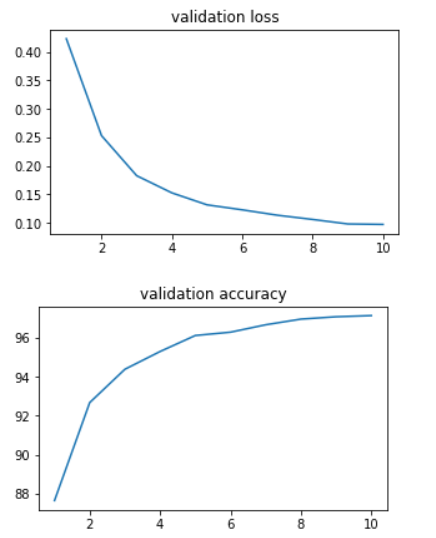
\includegraphics[scale=0.3]{2.png}
    \caption{Caption}
    \label{fig:1}
\end{figure}




\subsection{修改epoch}
从10个epochs修改到20个和5个。

\subsection{实验结果}

如图\ref{fig:1}所示
\begin{figure}[H]
    \centering
    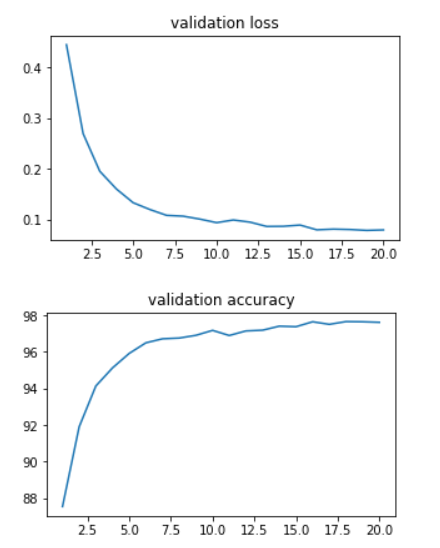
\includegraphics[scale=0.3]{4.png}
    \caption{Caption}
    \label{fig:1}
\end{figure}

\section{实验比对}

\begin{table}[!htbp]
    \centering
    \begin{tabular}{|c|c|c|c|c|c|c|}
    \hline
    $hidden_layer$&$dropout$&$epochs$&$acc$\\
    \hline
    1&0.2&5&0.9325\\
    \hline
    1&0.2&10&0.9451\\
    \hline
    1&0.2&20&0.9632\\
    \hline
    2&0.2&5&0.9592\\
    \hline
    2&0.2&10&0.9713\\
    \hline
    2&0.2&20&0.9766\\
    \hline
    2&0.3&5&0.9462\\
    \hline
    2&0.3&10&0.9633\\
    \hline
    2&0.3&20&0.9652\\
    \hline
    \end{tabular}
    \caption{实验结果比对}
  \end{table}

%----------------------------------------------------------------

%----------------------------------------------------------------
\bibliographystyle{plain}
\end{document}
